\label{sec:negative}
For our investigation of the negative coefficient situation we consider a simplified version of the Kuramoto oscilator. Specifically we assume that all oscilators have the same basic frequency $\omega_i$, which we just call $\omega$. We also assume that there is no external driver to the system, i.e. $b_i = 0$. This simplifies the system of ODEs to: 

\[
\dot{\theta_i} = \omega + \sum_{j = 0}^{N}{A_{i, j}\sin({\theta_j - \theta_i})}
)\]

Furthermore we assume that all coefficients in the matrix $A$ are either $-1$ or $0$. We can thus see $A$ as the negative of an adjacency matrix of a graph. Here each oscilator is considered as a node of a graph and an edge can be interpreted as $A$ having a $-1$ in the appropriate place. 

\subsection{The 2-oscilator system}

The first situation we consider is the case of only $2$ oscilators. It is obvious that if the oscilators are not connected through an edge, no synchronization occurs. Thus the only situation of interest is the case where they are connected through an edge, i.e. 
\[
  A = \left( \begin{array}{cc} 0 & -1\\ -1 & 0 \end{array} \right)
\]
We have simulated this situation with random initial values for the oscilators. As can be seen from the typical result in Figure~\ref{fig:negative_2_osc} the two oscilators lock to the same frequency but have a phase shift of $\pi$, i.e. they are in anti-phase. We observed that this behaviour occurs independent of the initial values. This behaviour stems from the fact that the two oscilators are influencing each other with equal negative coefficients and thus want to oscilate as far away from each other as possible. 

\begin{figure}[h]
  \centering
  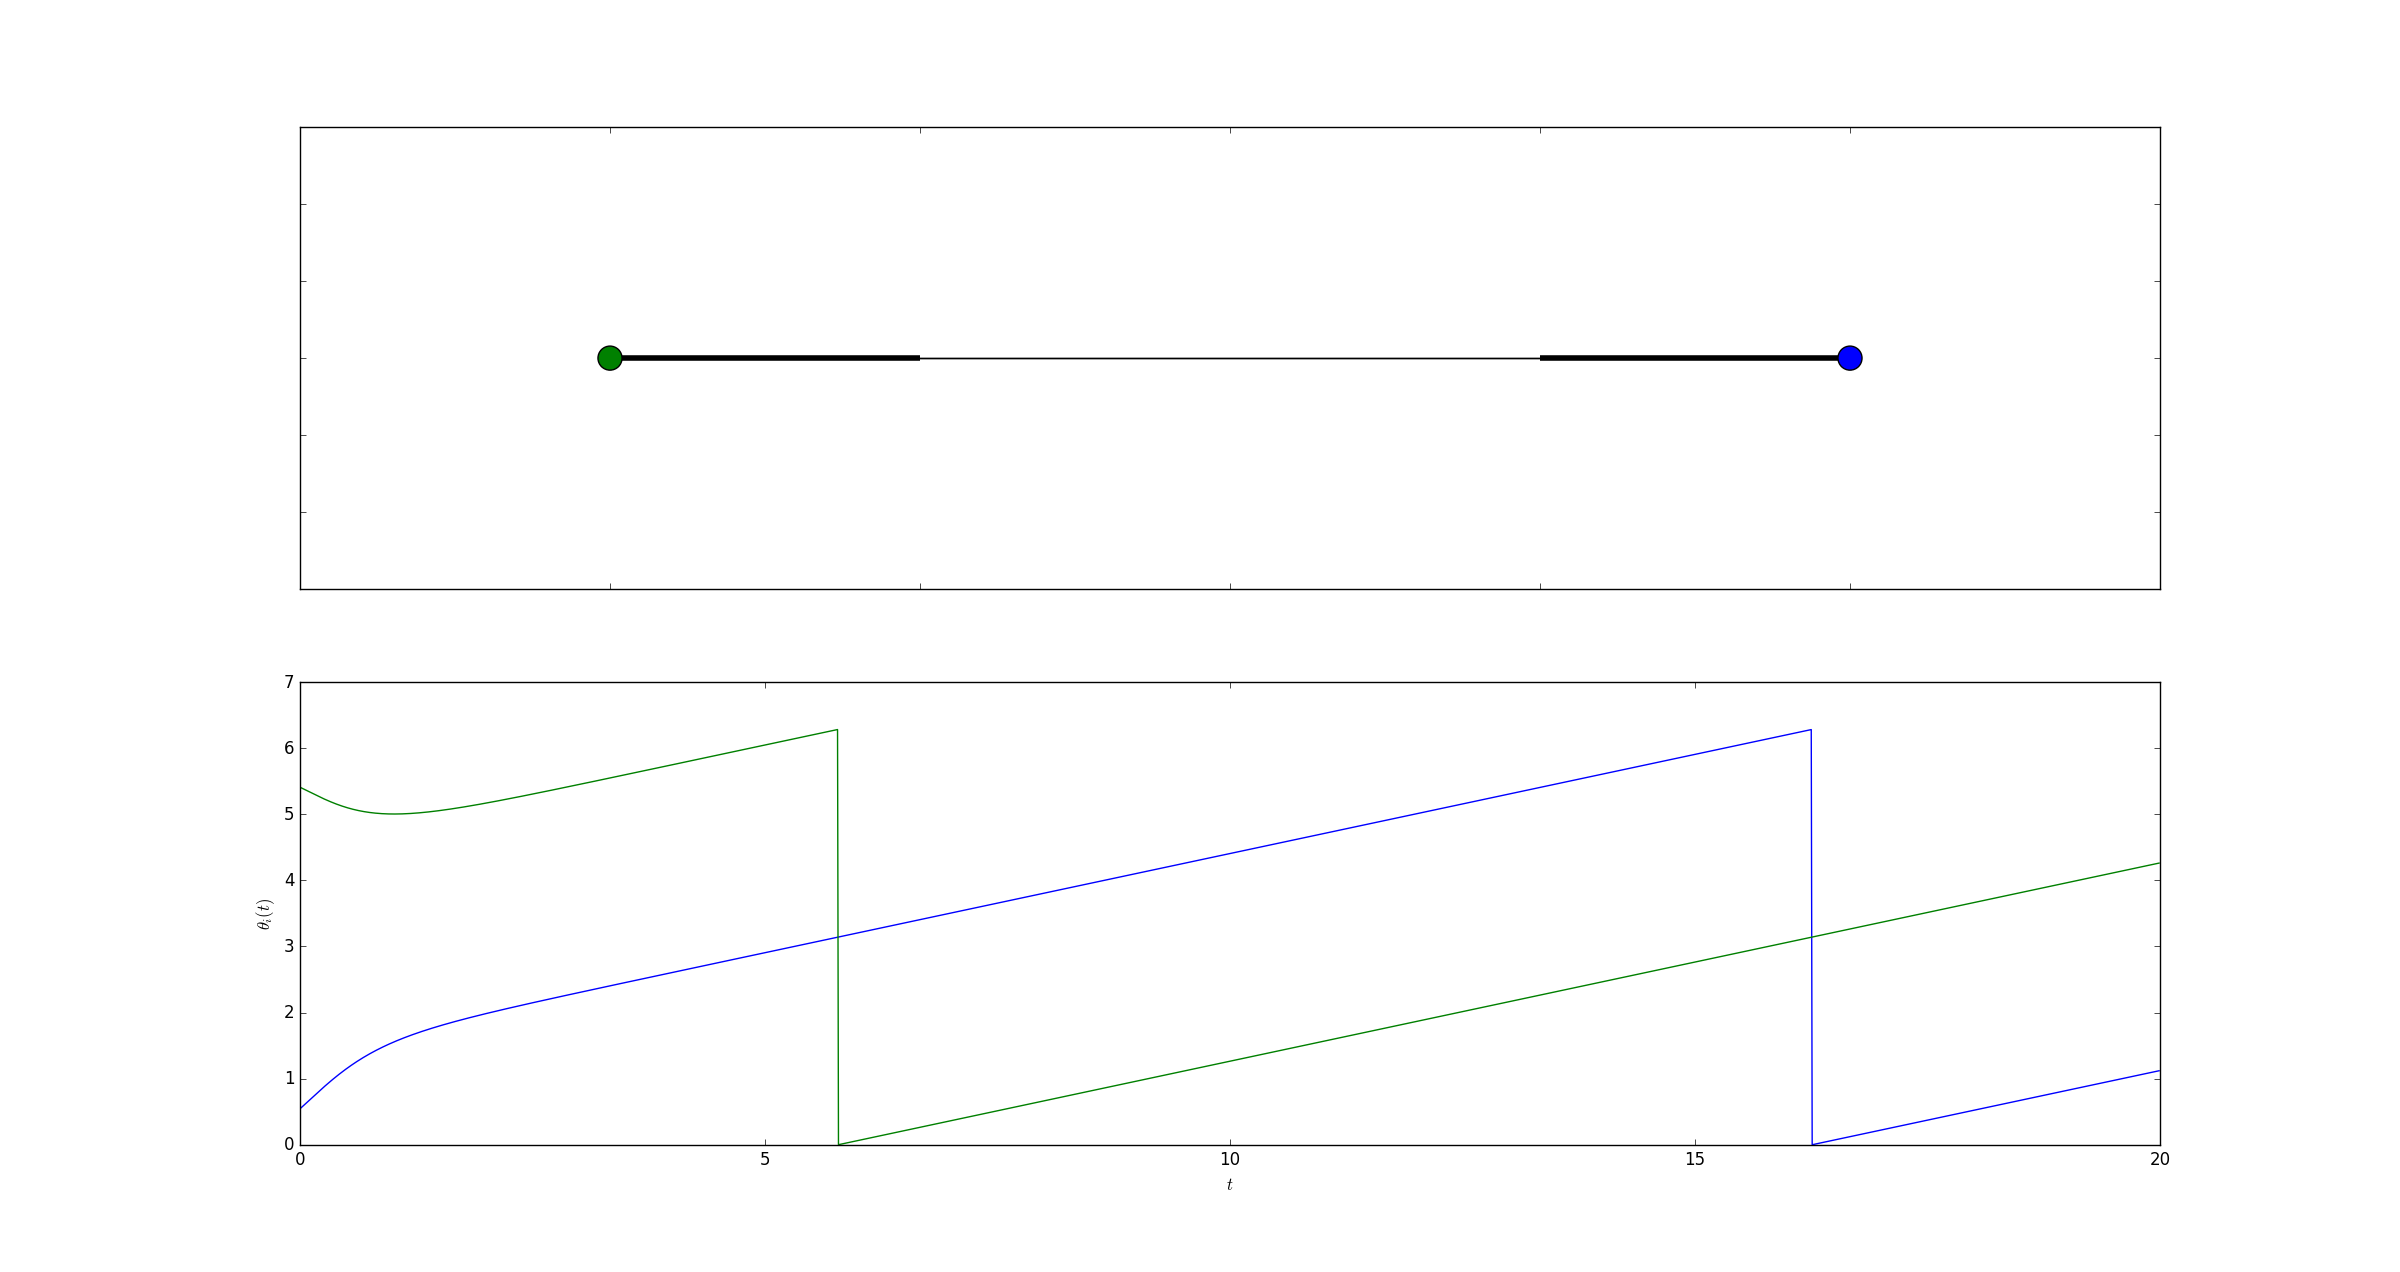
\includegraphics[width=\textwidth]{imgs/simple_2_osc}
  \caption{Simulation of a simplified 2 oscilator Kuramoto system with $\omega = 0.3$ and random initial values. $A$ is given by the negative of the adjacency matrix of the associated graph topology which can be seen in the upper part of the figure. The behaviour of the oscilators over time can be seen in the lower part. }
  \label{fig:negative_2_osc}
\end{figure}

\subsection{Oscilators on a line}

Next we want to expand this behaviour to the situation of several oscilators on a line. In this sense, that refers to the situation where $N$ oscilators are ordered linearly and each oscilator is only connected to the next and previous in the line with the exception of the ones at either end of the line. The associated matrices $A$ to these situations are $0$ except as two bands above and below the diagonal.  

In the case of three oscilators the adjacency matrix is given by
\[
  A_3 = \left( \begin{array}{ccc}
  0  & -1 &  0\\ 
  -1 &  0 & -1
  \end{array} \right)
\] 
and in the case of 10 oscilators it is given by
\[
  A_{10} = \left( \begin{array}{cccccccccc}
  0 & -1 & 0 & 0 & 0 & 0 & 0 & 0 & 0 & 0 \\
  -1 & 0 & -1 & 0 & 0 & 0 & 0 & 0 & 0 & 0 \\
  0 & -1 & 0 & -1 & 0 & 0 & 0 & 0 & 0 & 0 \\
  0 & 0 & -1 & 0 & -1 & 0 & 0 & 0 & 0 & 0 \\
  0 & 0 & 0 & -1 & 0 & -1 & 0 & 0 & 0 & 0 \\
  0 & 0 & 0 & 0 & -1 & 0 & -1 & 0 & 0 & 0 \\
  0 & 0 & 0 & 0 & 0 & -1 & 0 & -1 & 0 & 0 \\
  0 & 0 & 0 & 0 & 0 & 0 & -1 & 0 & -1 & 0 \\
  0 & 0 & 0 & 0 & 0 & 0 & 0 & -1 & 0 & -1 \\
  0 & 0 & 0 & 0 & 0 & 0 & 0 & 0 & -1 & 0
  \end{array} \right)
\]
The typical behaviour of such systems can be seen in Figures~\ref{fig:line_3} and \ref{fig:line_10} respectively. The behaviour naturally extends the behaviour of the 2 oscilator systems above: Neighbouring oscilators are in exact anti-phases. Experiments showed this behaviour to be independent of initial values and the number of oscilators, although the higher the number of oscilators, the longer the system needs to reach this state. 

\begin{figure}[h]
  \centering
  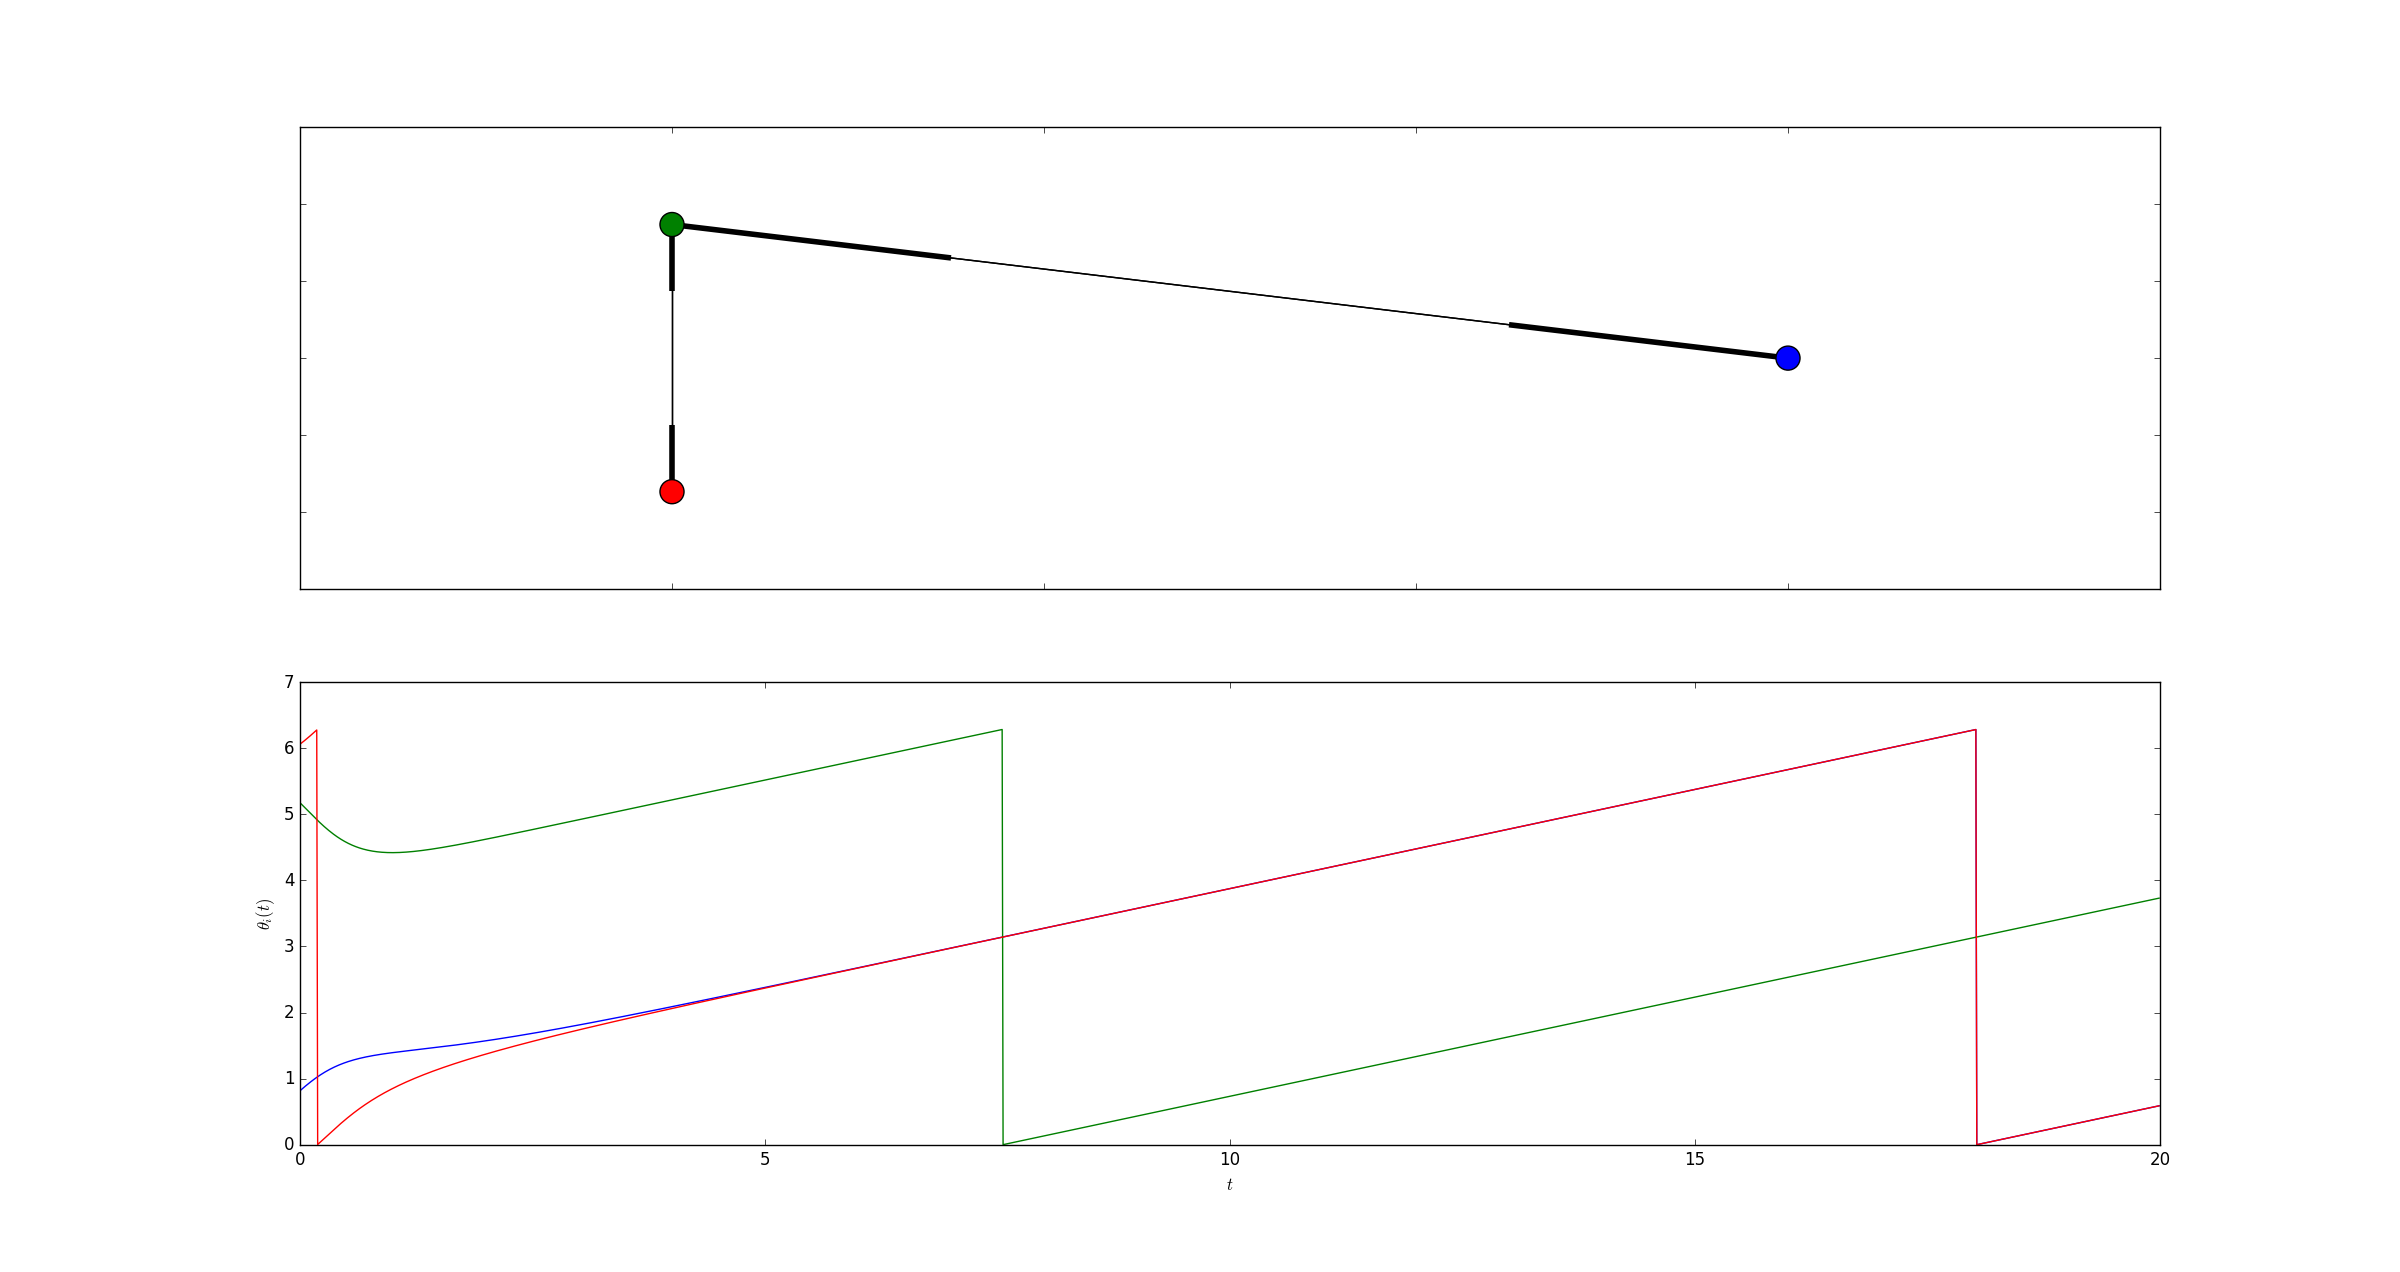
\includegraphics[width=\textwidth]{imgs/line_3}
  \caption{Simulation of a 3 oscilators-on-a-line Kuramoto oscilator system with $\omega = 0.3$ and random initial values. Again $A$ is given by the negative of the adjacency matrix of the associated graph topology. }
  \label{fig:line_3}
\end{figure}

\begin{figure}[h]
  \centering
  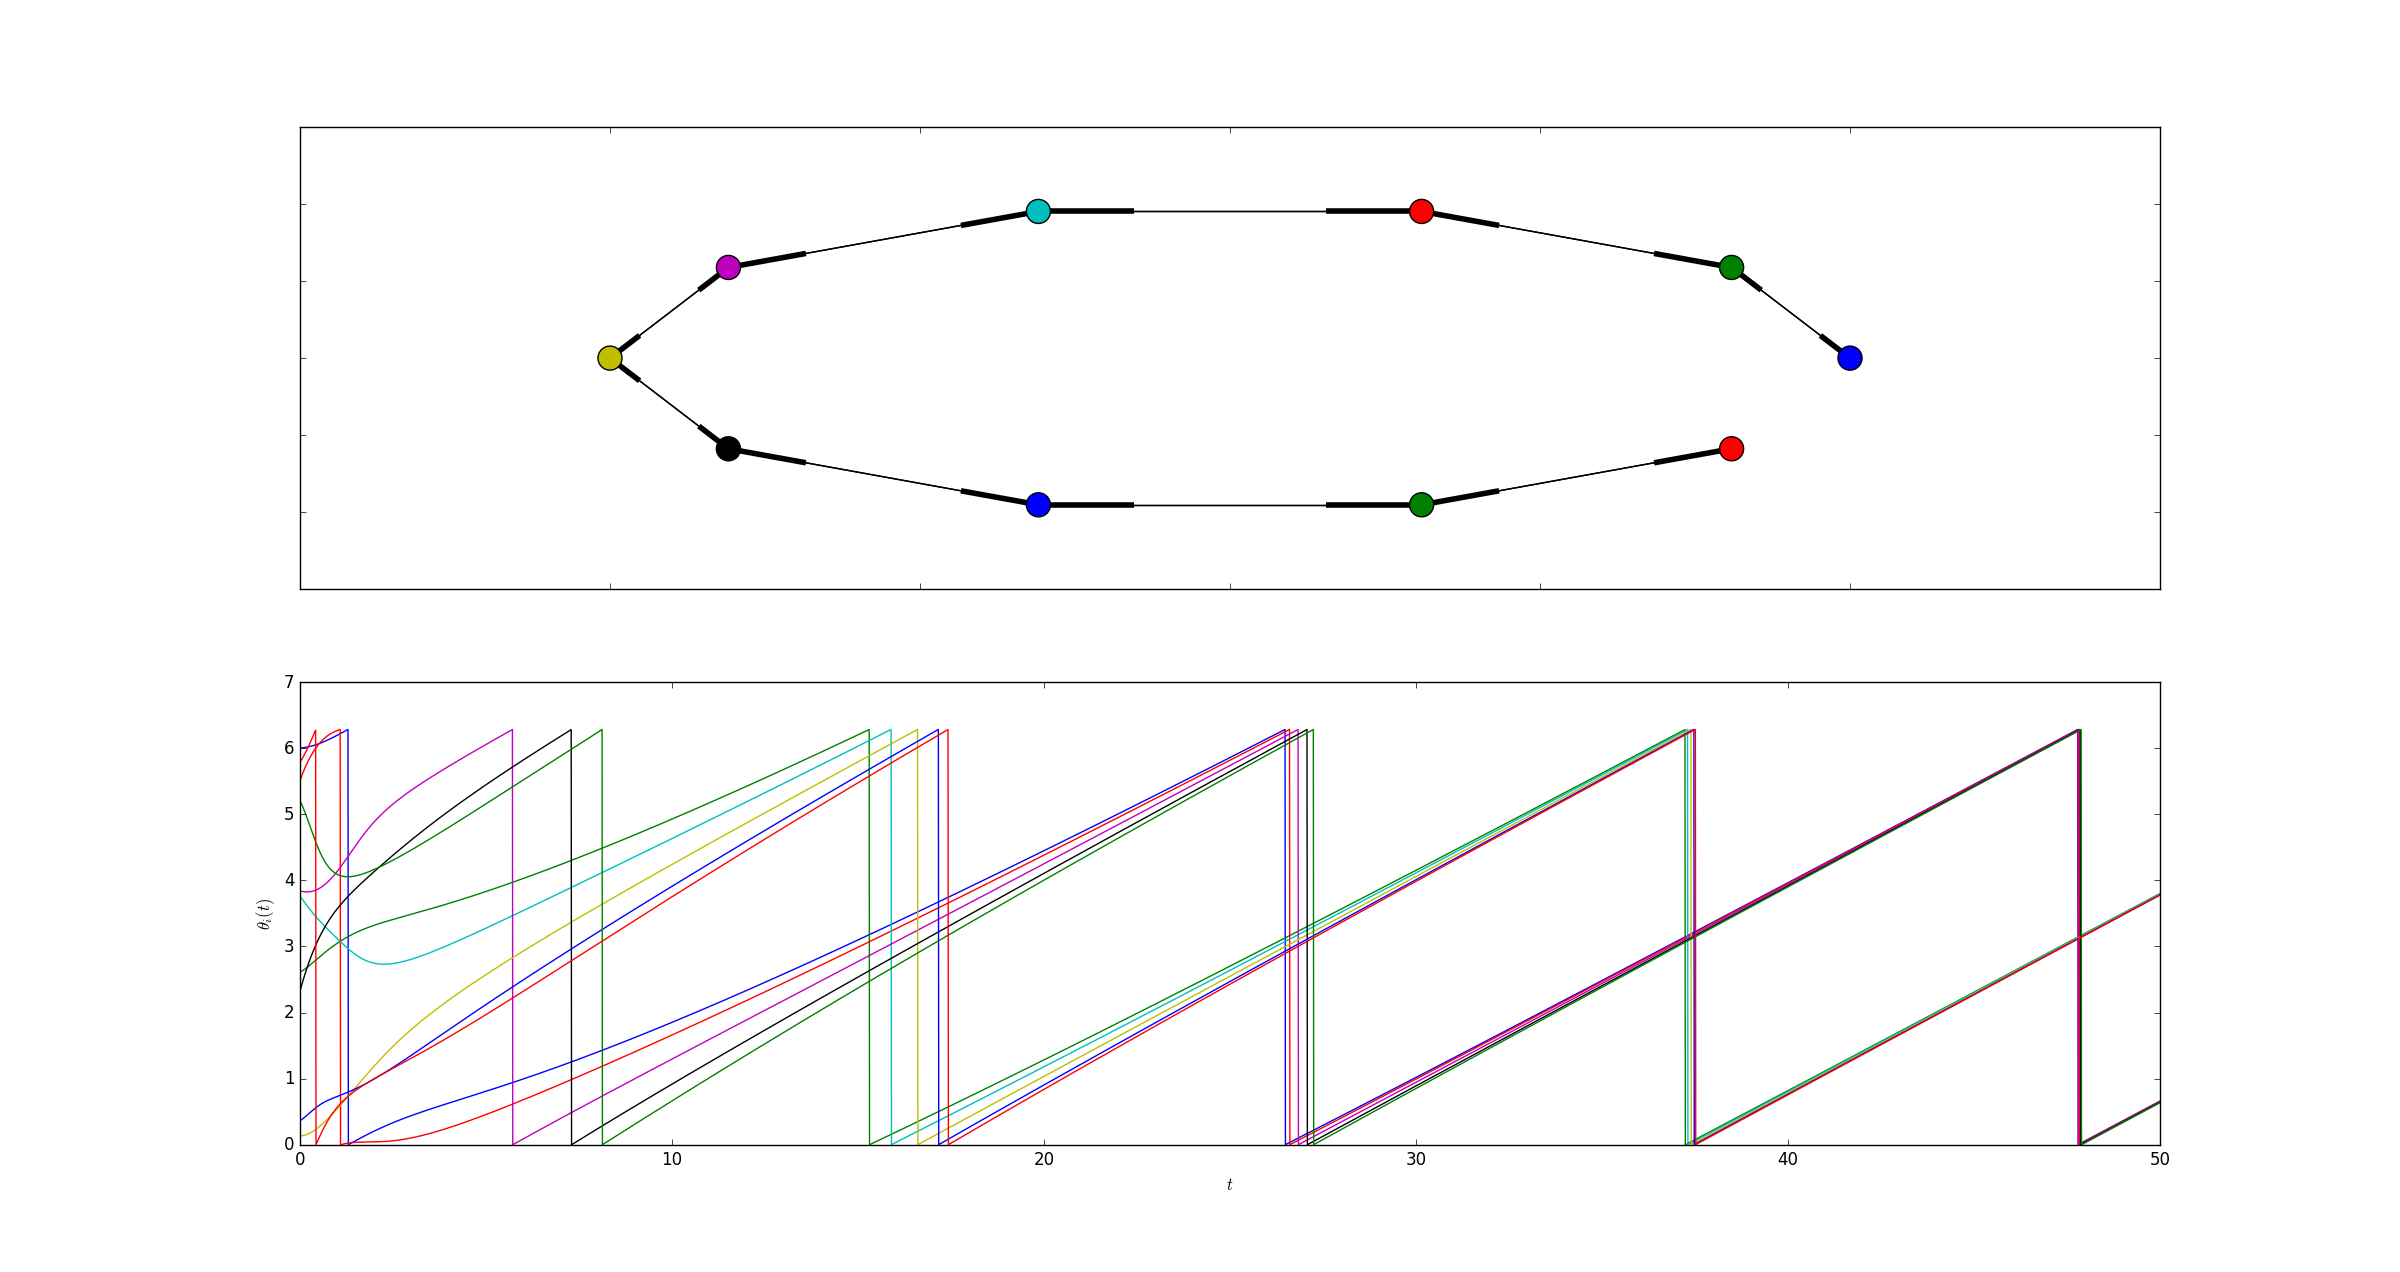
\includegraphics[width=\textwidth]{imgs/line_10}
  \caption{Simulation of a 10 oscilators-on-a-line Kuramoto oscilator system with $\omega = 0.3$ and random initial values. Again $A$ is given by the negative of the adjacency matrix of the associated graph topology. }
  \label{fig:line_10}
\end{figure}

\subsection{Oscilators on a Circle System}

The final patterns we observed were patterns in the case of $N$ oscilators on a cycle. This graph looks very similar to the oscilators-on-a-line situation except that the first and last nodes are connected via an edge as well. We have again simulated the system and in this situation we came to interesting results. In the case of $3$ oscilators on a cycle (which can be seen in Figure~\ref{fig:circle_3}) the behaviour is obvious: The oscilators synchronize with phase-shits of exactly $\frac{2 \pi}{3}$. 

\begin{figure}[h]
  \centering
  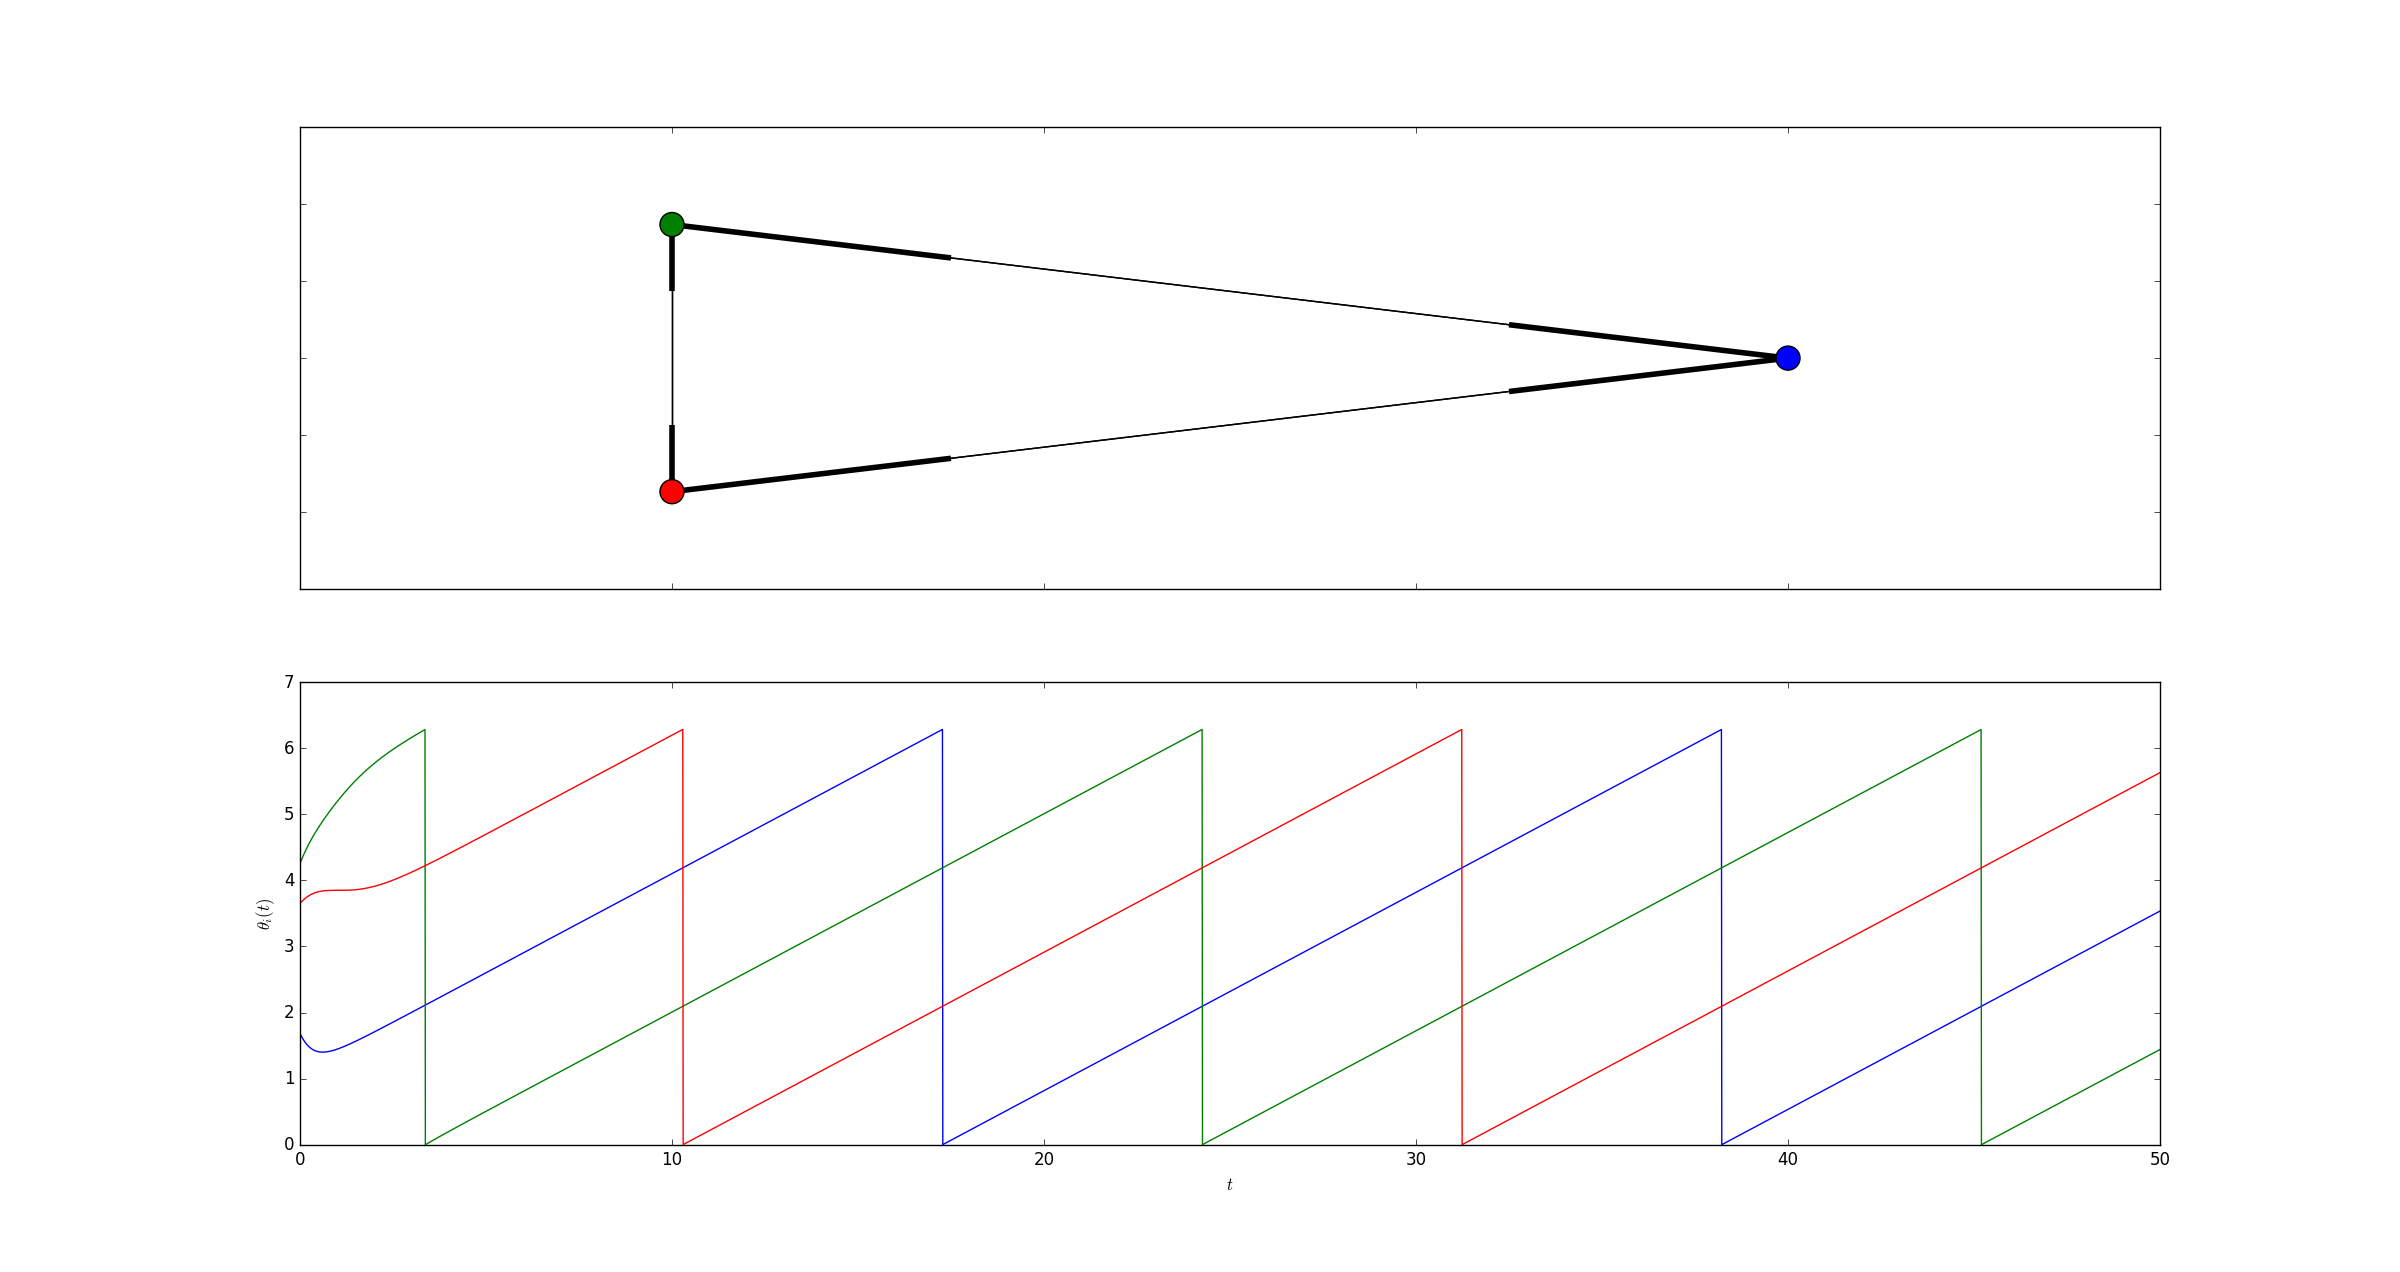
\includegraphics[width=\textwidth]{imgs/circle_3}
  \caption{Simulation of a 3 oscilators-on-a-circle Kuramoto oscilator system with $\omega = 0.3$ and random initial values. Again $A$ is given by the negative of the adjacency matrix of the associated graph topology. }
  \label{fig:circle_3}
\end{figure}

The behaviour becomes more interesting however if we choose a different number of oscilators, for example $6$. In this case we observed three different situations with three different kinds of phase shifts: Either phase shifts of $\pi$ (nodes with distance 2 were exactly in phase, see Figure~\ref{fig:circle_6a}), phase shifts of $\frac{2 \pi}{3}$ (nodes with distance 3 were exactly in phase, see Figure~\ref{fig:circle_6b}) or phase shifts of $\frac{2 \pi}{6}$ (see Figure~\ref{fig:circle_6c}). The last of these patterns could only be produced artificially by choosing the desired situation as initial values and proved to be very unstable. 

\begin{figure}[h]
  \centering
  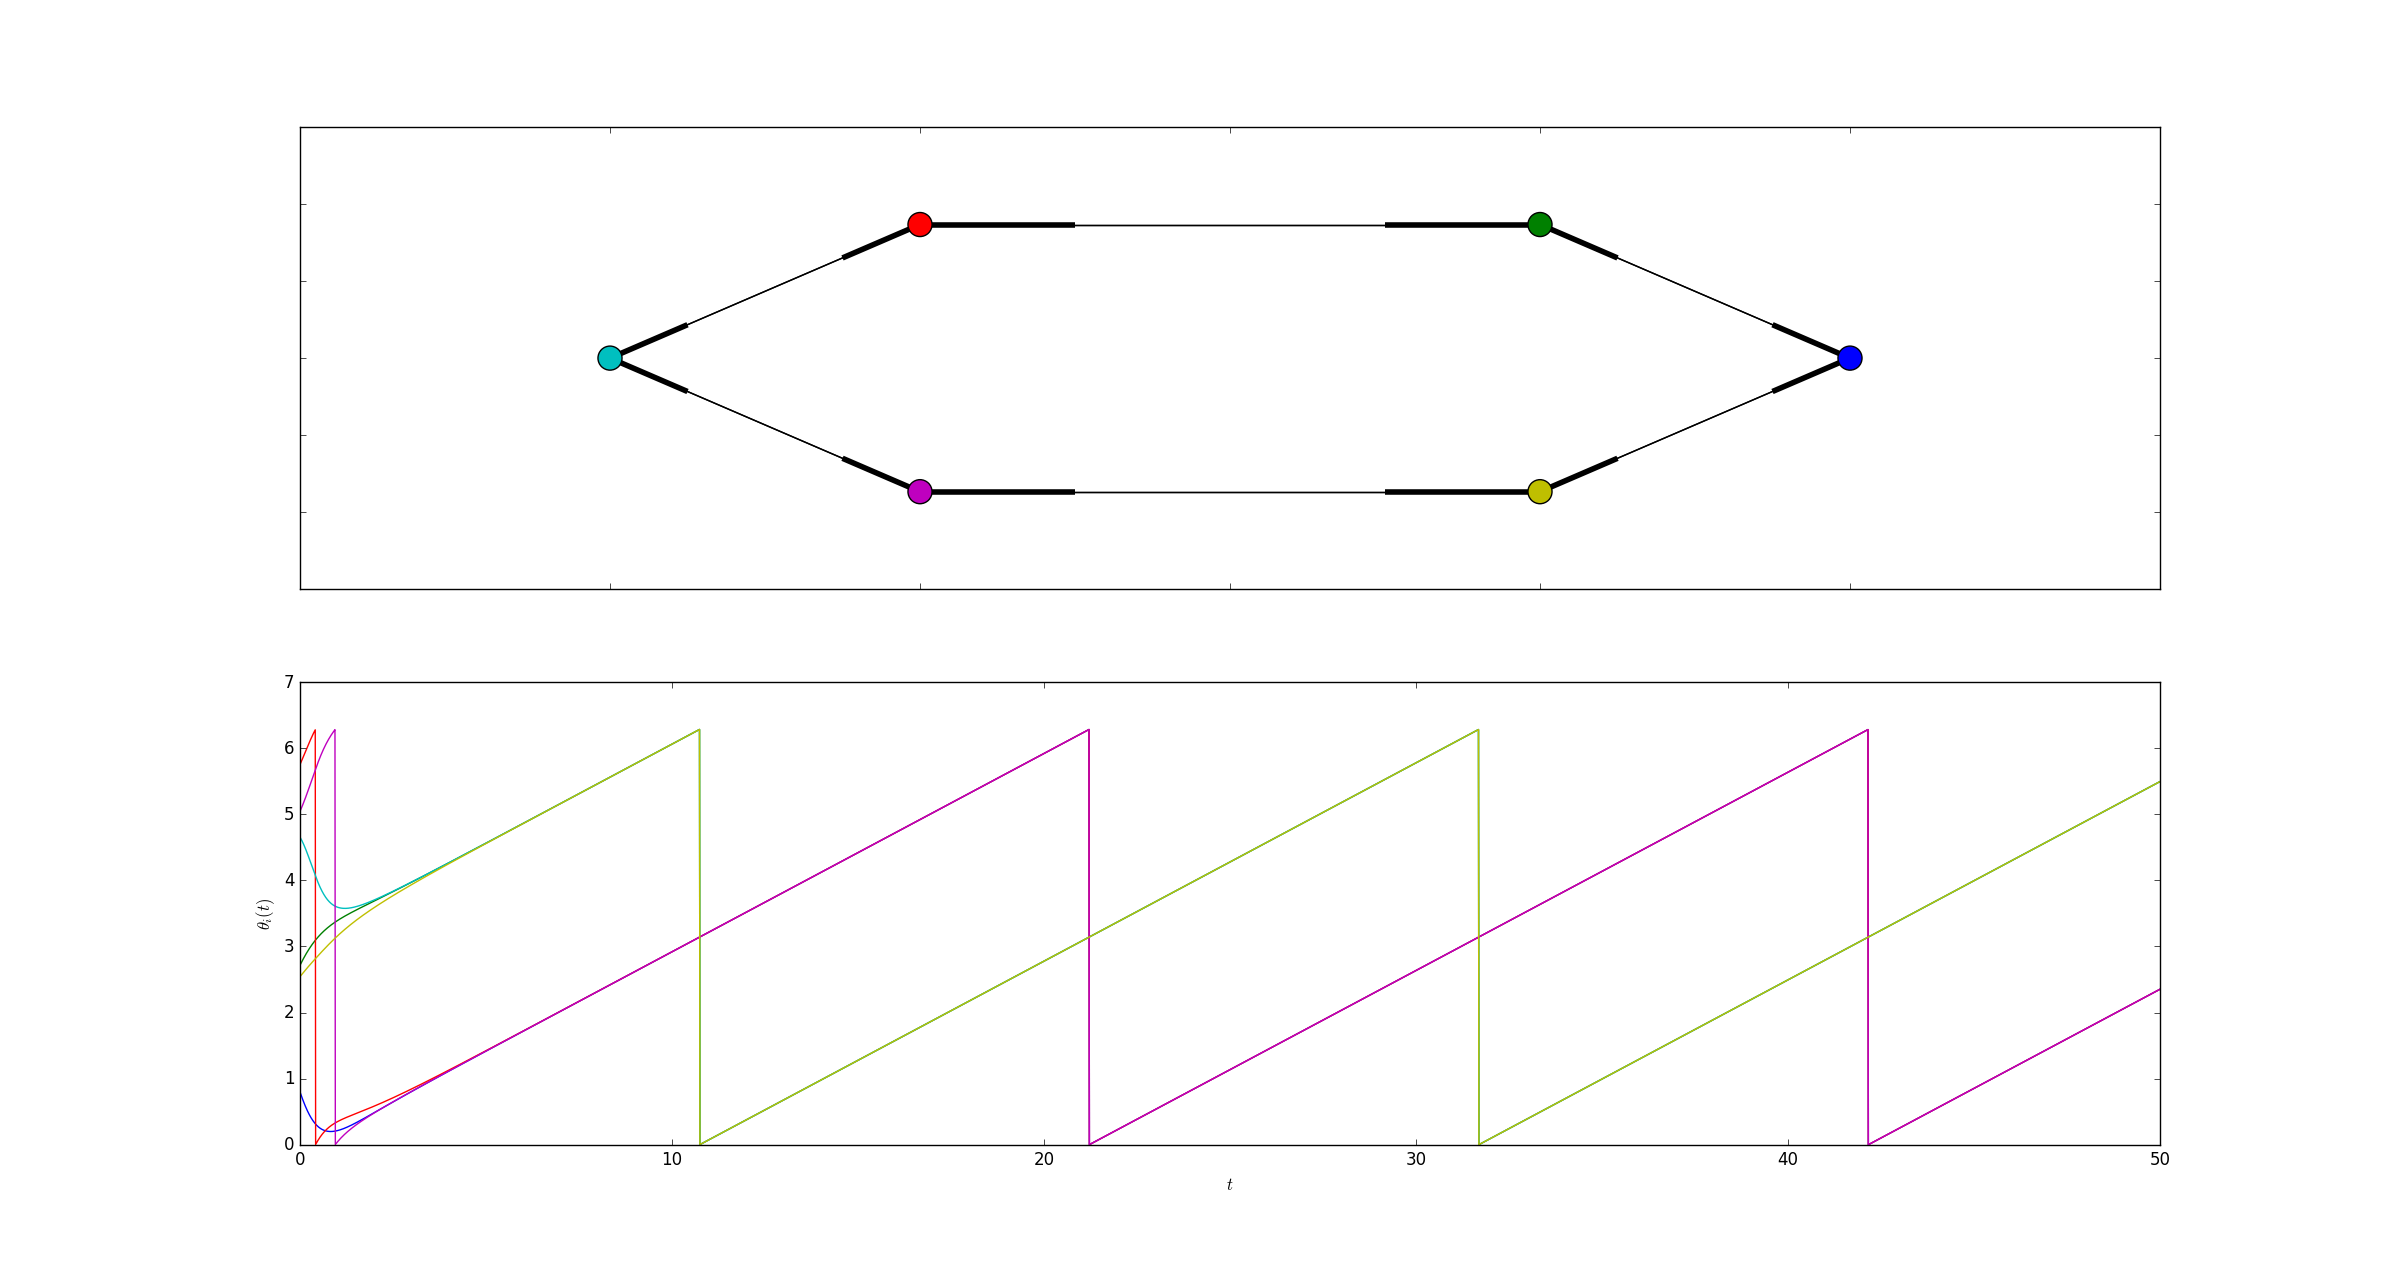
\includegraphics[width=\textwidth]{imgs/circle_6a}
  \caption{Simulation of a 6 oscilators-on-a-circle Kuramoto oscilator system with $\omega = 0.3$ and random initial values producing a pattern of neighbouring oscilators being exactly anti-phase}
  \label{fig:circle_6a}
\end{figure}

\begin{figure}[h]
  \centering
  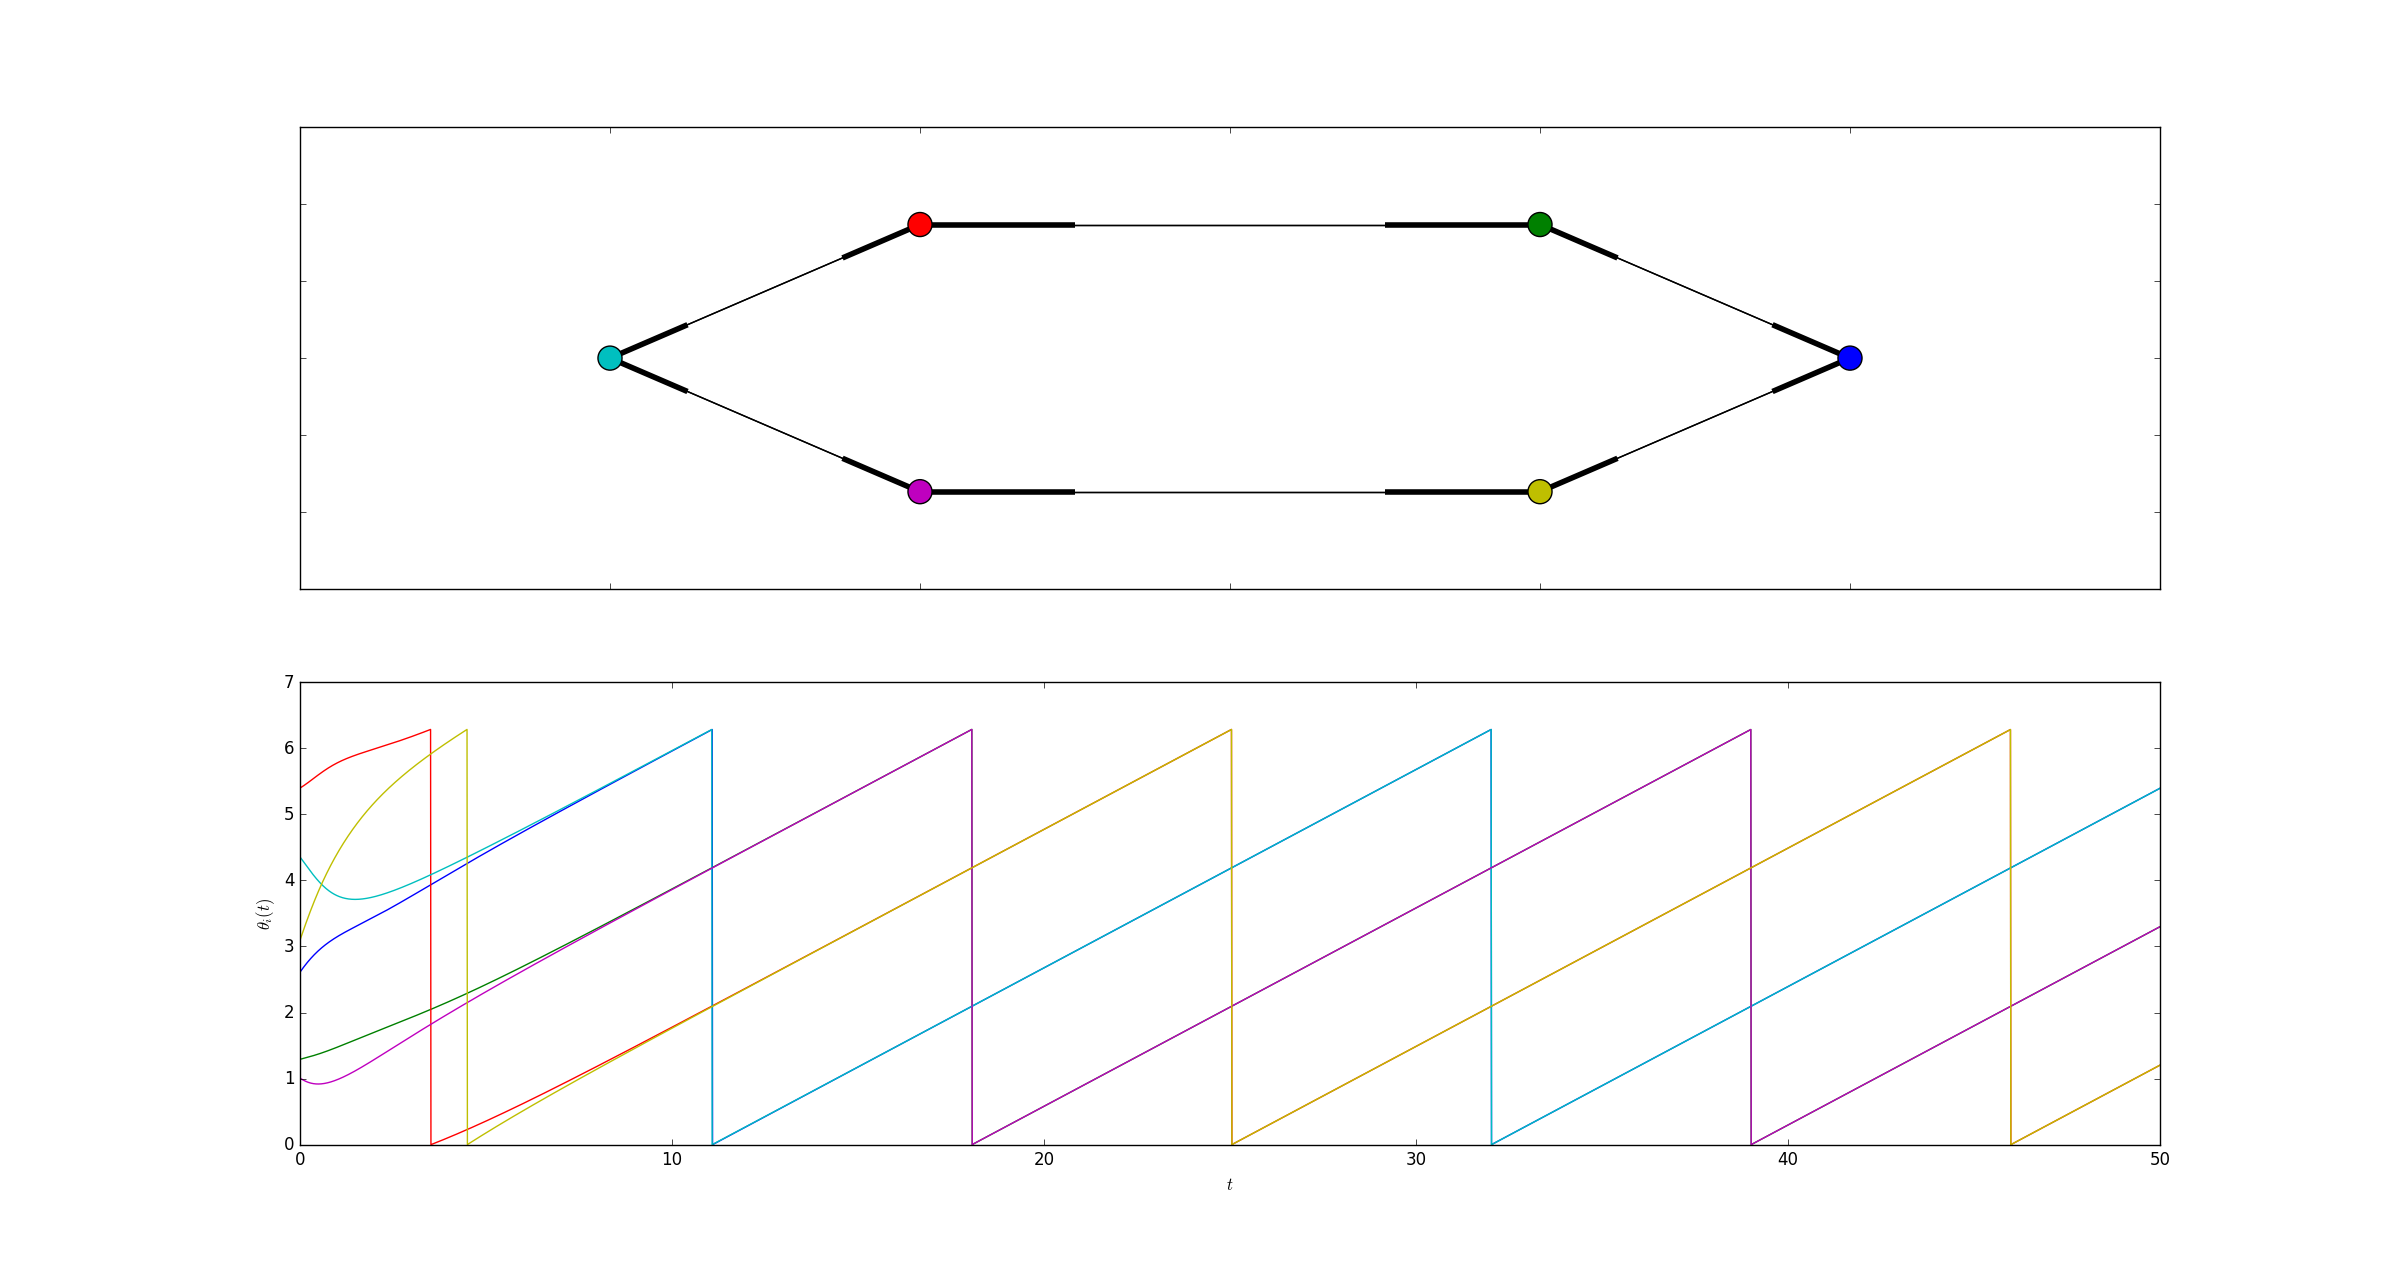
\includegraphics[width=\textwidth]{imgs/circle_6b}
  \caption{Simulation of a 6 oscilators-on-a-circle Kuramoto oscilator system with $\omega = 0.3$ and random initial values priducing a pattern of every 3 oscilators being in sync. }
  \label{fig:circle_6b}
\end{figure}

\begin{figure}[h]
  \centering
  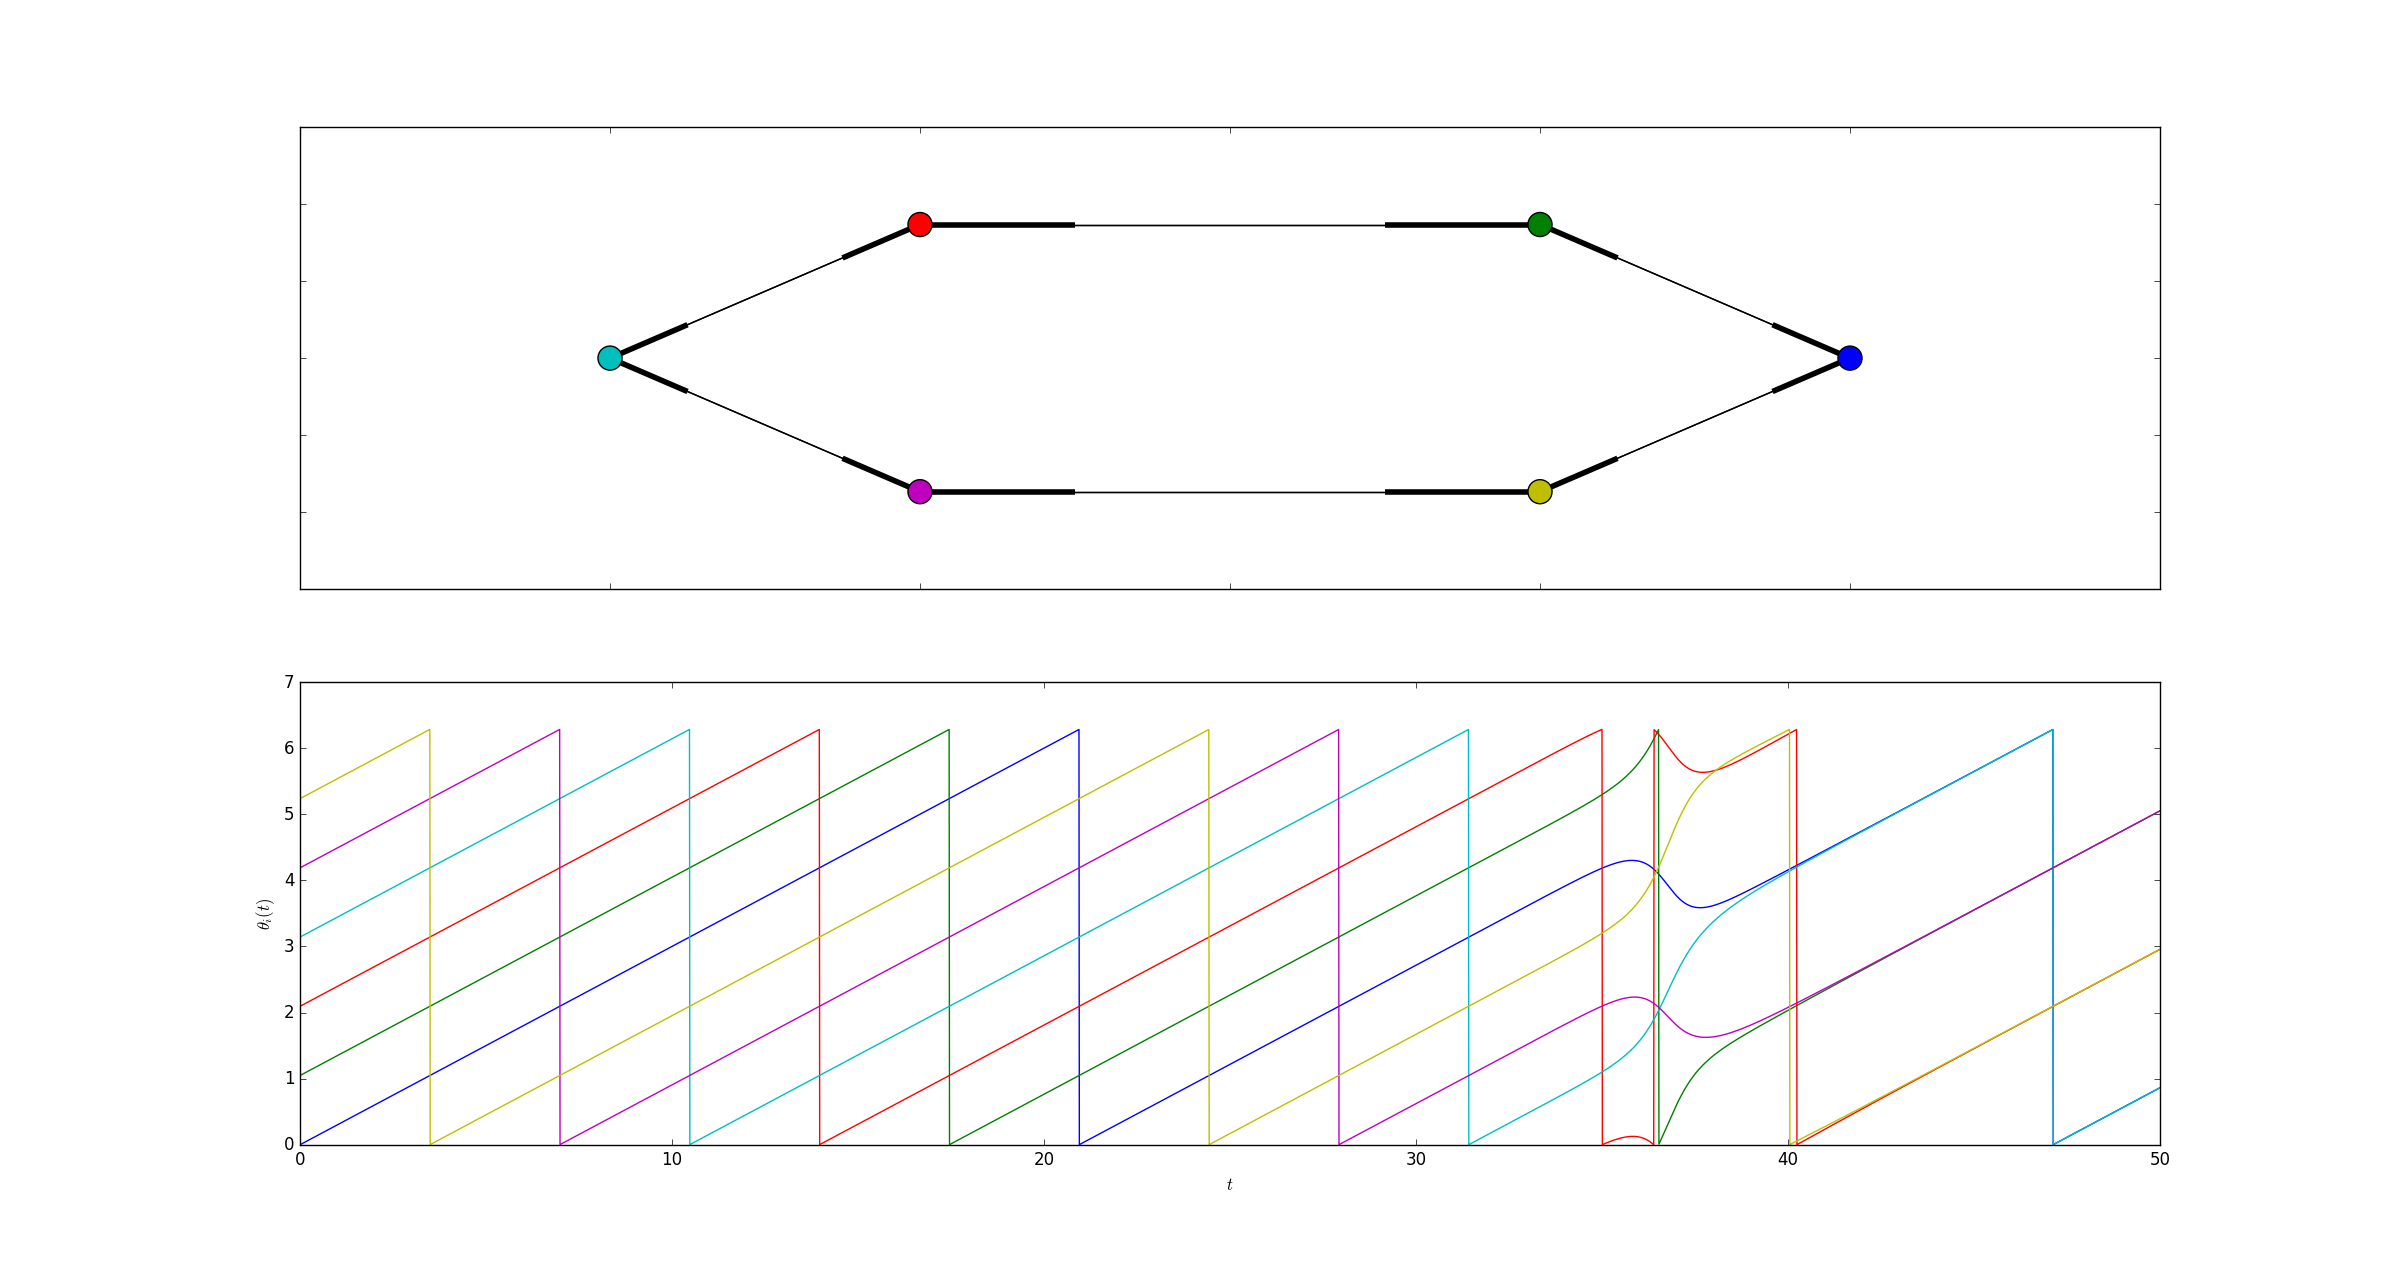
\includegraphics[width=\textwidth]{imgs/circle_6c}
  \caption{Simulation of a 6 oscilators-on-a-circle Kuramoto oscilator system with $\omega = 0.3$ and specific initial values producing an unstable pattern of oscilators being evenly spaced out in phase shifts. }
  \label{fig:circle_6c}
\end{figure}

From these patterns we can deduce that the possible patterns in the general case of $N$ oscilators-on-a-circle depends on the divisors of $N$. Since each oscilator wants to be as far away from its neighbours as possible, they space out equally with respect to their phase shifts. However since each oscilator has to be in phase with itself, the sum of all phase shifts around the cycle must be a multiple of $2\Pi$. Thus for each divisor of $N$ we get a different pattern, which is exactly what we observed. 